\section{Аналитическая часть}

Проблемы эмулятора:
\begin{itemize}[leftmargin=1.6\parindent]
	\item[---] управление кэшем транслированного кода;
	\item[---] выделение регистров;
	\item[---] оптимизация условных блоков;
	\item[---] direct block chaining????? а по русски;
	\item[---] управление памятью;
	\item[---] поддержка самоизменяемого кода;
	\item[---] поддержка исключений;
	\item[---] поддержка аппаратных прерываний.
\end{itemize}

\subsection{QEMU}

кему это круто написать что это такое

\subsubsection{Сворачивание и оптимизация тривиальных выражений}

В qemu определены свои опкоды, каждый из них может по своему сворачиваются. TCG ops (специальные операции TCG) оптимизируются и затем выполняются на хосте, таким образом портировать TCG становится проще. Операции поддерживаются над 32 и 64 битными целыми числами, указатели определены как алиас над соответствующим целым числом.

Пример операции TCG:\\
\texttt{add\_i32 t0, t1, t2  (t0 <- t1 + t2)}

Одной из оптимизаций является игнорирование бессмысленных операций, например операция:\\
\texttt{and\_i32 t0, t0, \$0xffffffff\\}
выполняться не будет

Подавляются неиспользуемые перемещения данных, например из трех операций:\\
\texttt{add\_i32 t0, t1, t2\\
add\_i32 t0, t0, \$1\\
mov\_i32 t0, \$1\\}
выполнится только последняя.

(оптимизации над инструкциями реализованы в файле tcg/optimize.c)

\subsubsection{Состояние процессора и блоки трансляции}

Блоком трансляции называется часть кода до момента изменения состояния процессора которое нельзя выяснить на этапе трансляции (например, некоторое ветвление).

Каждый регистр проверяется на используемость в определенном блоке трансляции, если регистр не используется в блоке трансляции связанные с ним операции оптимизируются, так как значения этих регистров (и связанное с ними состояние процессора) за блок не могут измениться. Если состояние виртуального процессора меняется, такой блок не будет выполняться пока состояние процессора не будет соответствовать необходимому для блока (например, другой уровень привилегий).

Пример: если на x86 регистры SS, DS и SS содержат в себе 0, транслятор не будет генерировать для них смещение.

\subsubsection{Блок чейнинг??}

После выполнения блока трансляции QEMU ищет следующий блок, для этого используется PC (эмулируемый program counter) и другая информация о статусе процессора (например регистр CS). (реализовано в функции tb\_lookup в файле accel/tcg/cpu-exec.c)

Сначала блок ищется в кэше трансляции, если он там не найден он достается из хэш-таблицы и добавляется в кэш.

Для этого нужно выйти из цикла выполнения блока, пройти через эпилог процедуры, найти следующий блок, запустить его, пройдя через пролог процедуры. В качестве оптимизации предлагается связывать несколько блоков трансляции напрямую.

Для этого в конце блока вызывается tcg\_gen\_lookup\_and\_goto\_ptr(), он в свою очередь вызывает helper\_lookup\_tb\_ptr который ищет нужный блок и генерирует инструкцию goto\_ptr, которая либо продолжит управление в нужном блоке, либо вернется в основной цикл. (пример вызова для i386 в файле target/i386/tcg/translate.c в функции do\_gen\_eob\_worker)

Еще одной оптимизацией является оптимизация ветвления. Если ветвление происходит напрямую, в пределах одной страницы QEMU выполняет поиск блока трансляции на который будет произведено ветвление, а затем сохраняет его адрес в транслированном коде. Таким образом при следующем выполнении этого блока нет необходимости в поиске следующего блока.

\subsubsection{Поддержка самомодифицирующегося кода}

Самомодифицирующийся код на x86 представляет особую проблему, так как нет механизма оповещения о изменении кода. При запуске в режиме пользователя QEMU помечает все страницы с транслированным кодом как защищенные от записи, при попытке записи в них поднимается сигнал SEGV, допускается запись, обнуляются все транслированные страницы и связь блоков. При запуске эмуляции системы программный MMU выполняет защиту от записи.
Для эффективного выполнения этих операций хранится связанный список всех блоков трансляции и связей блоков.

\subsubsection{Эмуляция MMU}

Каждый доступ к памяти проходит через MMU, в нем адреса преобразуются из виртуальных к реальным. Для ускорения трансляции адреса хранится TLB-кэш.

Все блоки трансляции в кэше индексируются при помощи их физического адреса, таким образом нет необходимости очищать кэш при смене страницы.

\subsection{box64}

box64 это норм написать что такое

В отличии от QEMU box64 не может эмулировать полную систему (то есть на нем нельзя, например, запустить Windows), однако можно запускать linux-приложения собранные под x86\_64.

\subsubsection{Трансляция}

Трансляция в box64 производится при помощи dynarec или при помощи эмулятора процессора. Для ARM реализован полноценный dynarec, для всех остальных архитектур написан общий эмулятор процессора интерпретирующий инструкции. Dynarec написан на C, на ассемблере реализованы пролог и эпилог.

\subsubsection{Поддержка родных библиотек}

Главным механизмом позволяющим добиться хорошей производительности является использование родных для архитектуры библиотек. Таким образом в графически требовательных приложениях производительность близка к 100\%, однако в приложениях не использующие сторонние библиотеки (то есть полностью транслируемые) производительность около 50\%.

При эмуляции Quake 3 (графического приложения с большим количеством повторно используемых функций) производительность была около 85\%.

Необходимые для работы приложения библиотеки либо транслируются, либо используется родная библиотека (в таком случае производительность выше). Вызовы функций перехватываются для вызова родных функций. 

В ELF содержатся специальные символы называемые перемещениями (relocations), они используются при линковке для установки адреса необходимой функции. При вызове родной функции в качестве адреса выставляется адрес заранее подготовленного кода, он состоит из CC 53 43 и двух указателей. Первый указатель рассматривается как указатель на оберточную функции, а второй как указатель на обертываемую (родную) функцию. Оберточной функции передается структура с состоянием процессора и указатель на вызываемую функцию, эта структура распаковывается и вызывается переданная функция. По завершению работы оберточная функции завершается через ret или retn.

Поиск необходимой функции осуществляется при помощи файлов находящихся в src/wrapped, их необходимо определять в ручную, так как названия функций не сохраняются после компиляции программы. Сигнатура функции состоит из символов определяющих тип возвращаемого значения и типов аргументов разделенных буквой F. Пример сигнатуры показан на рисунке \ref{fig:box64sig}.

\begin{figure}[hbtp]
	\centering
	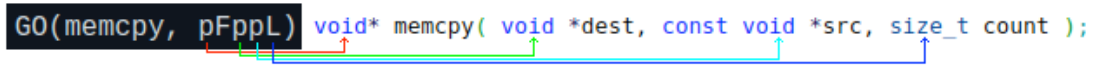
\includegraphics[width=\textwidth]{img/box64_sig.png}
	\caption{Пример сигнатуры функции memcpy}
	\label{fig:box64sig}
\end{figure}

После определения функция заносится в таблицу функций библиотеки, а затем находится при помощи разных методов (// посмотреть что за методы).

Одной из оптимизаций в box64, по сравнению с box86, является определение простых функций, такие функции не нуждаются в оберточной функции и вызываются напрямую, тем самым экономя время.

\subsubsection{Процесс трансляции}

Так же как и в QEMU код разбивается на блоки трансляции, блок заканчивается когда после нее нет других инструкций (например jump, call или ret) и когда на последнюю инструкцию не ссылается какое-либо ветвление из этого блока. Исключения: multi-bytes NOP are handled, а неизвестная инструкция останавливает процесс выполнения блока.

Каждый блок транслируется в 4 прохода:
\begin{itemize}[leftmargin=1.6\parindent]
	\item[---] Первый проход считает все количество транслируемых x86 инструкций. Для каждой инструкции выделяется память;
	\item[---] На втором проходе обрабатываются все инструкции ветвления, проверяется где находится адрес: в этом же блоке или в каком-либо другом. В случае если адрес находится в другом блоке его необходимо связать (// LinkNext() ?) с текущим. Также рассчитываются флаги, не нужные флаги предлагается не рассчитывать, так как инструкция может использовать/выставлять не все флаги;
	\item[---] На третьем проходе считается количество необходимых ARM инструкций в блоке;
	\item[---] На четвертом проходе генерируются необходимые инструкции.
\end{itemize}

После генерации блока он записывается в таблицу сгенерированных блоков в которой также содержится отображение эмулированных адресов в физические.

\subsubsection{JITs (mono) and self-modifying code.}

I'm doing something similar, yes. All pages from which x86 code has been translated are write protected. Once a write occurs, all blocks generated from this page are marked dirty, and the jump table from those blocks are invalidated (to avoid automatic jump from block to block to this one). Once x86 code wants to run a "dirty" block, a crc32 of the memory is runned and compared to the crc computed when creating the block. depending if it's the same or non, the block is marked as clean (and the page protected again) or deleted and a new one is generated (and the page also protected again)


\subsection{ДАЛЬШЕ МОЖНО НЕ ЧИТАТЬ}

Список:

\begin{itemize}[leftmargin=1.6\parindent]
	\item[---] первое;
	\item[---] второе;
	\item[---] пятое;
	\item[---] десятое.
\end{itemize}

Формула:

\begin{equation}
c^2 = a^2 + b^2
\end{equation}

Ссылаемся на рисунок \ref{fig:a1}. Информация из источника \cite{golang}.

\begin{figure}[hbtp]
	\centering
	
\includegraphics[width=\textwidth]{img/golang.png}
	\caption{Пример рисунка}
	\label{fig:a1}
\end{figure}

\begin{code}
	\captionof{listing}{Пример кода}
	\label{code:1}
	\inputminted
	[
	frame=single,
	framerule=0.5pt,
	framesep=20pt,
	fontsize=\small,
	tabsize=4,
	linenos,
	numbersep=5pt,
	xleftmargin=10pt,
	]
	{text}
	{code/main.go}
\end{code}

\pagebreak